\documentclass[]{book}
\usepackage{lmodern}
\usepackage{amssymb,amsmath}
\usepackage{ifxetex,ifluatex}
\usepackage{fixltx2e} % provides \textsubscript
\ifnum 0\ifxetex 1\fi\ifluatex 1\fi=0 % if pdftex
  \usepackage[T1]{fontenc}
  \usepackage[utf8]{inputenc}
\else % if luatex or xelatex
  \ifxetex
    \usepackage{mathspec}
  \else
    \usepackage{fontspec}
  \fi
  \defaultfontfeatures{Ligatures=TeX,Scale=MatchLowercase}
\fi
% use upquote if available, for straight quotes in verbatim environments
\IfFileExists{upquote.sty}{\usepackage{upquote}}{}
% use microtype if available
\IfFileExists{microtype.sty}{%
\usepackage{microtype}
\UseMicrotypeSet[protrusion]{basicmath} % disable protrusion for tt fonts
}{}
\usepackage[margin=1in]{geometry}
\usepackage{hyperref}
\hypersetup{unicode=true,
            pdftitle={Poverty and Inequality with Complex Survey Data},
            pdfauthor={Guilherme Jacob, Anthony Damico, and Djalma Pessoa},
            pdfborder={0 0 0},
            breaklinks=true}
\urlstyle{same}  % don't use monospace font for urls
\usepackage{natbib}
\bibliographystyle{apalike}
\usepackage{color}
\usepackage{fancyvrb}
\newcommand{\VerbBar}{|}
\newcommand{\VERB}{\Verb[commandchars=\\\{\}]}
\DefineVerbatimEnvironment{Highlighting}{Verbatim}{commandchars=\\\{\}}
% Add ',fontsize=\small' for more characters per line
\usepackage{framed}
\definecolor{shadecolor}{RGB}{248,248,248}
\newenvironment{Shaded}{\begin{snugshade}}{\end{snugshade}}
\newcommand{\KeywordTok}[1]{\textcolor[rgb]{0.13,0.29,0.53}{\textbf{{#1}}}}
\newcommand{\DataTypeTok}[1]{\textcolor[rgb]{0.13,0.29,0.53}{{#1}}}
\newcommand{\DecValTok}[1]{\textcolor[rgb]{0.00,0.00,0.81}{{#1}}}
\newcommand{\BaseNTok}[1]{\textcolor[rgb]{0.00,0.00,0.81}{{#1}}}
\newcommand{\FloatTok}[1]{\textcolor[rgb]{0.00,0.00,0.81}{{#1}}}
\newcommand{\ConstantTok}[1]{\textcolor[rgb]{0.00,0.00,0.00}{{#1}}}
\newcommand{\CharTok}[1]{\textcolor[rgb]{0.31,0.60,0.02}{{#1}}}
\newcommand{\SpecialCharTok}[1]{\textcolor[rgb]{0.00,0.00,0.00}{{#1}}}
\newcommand{\StringTok}[1]{\textcolor[rgb]{0.31,0.60,0.02}{{#1}}}
\newcommand{\VerbatimStringTok}[1]{\textcolor[rgb]{0.31,0.60,0.02}{{#1}}}
\newcommand{\SpecialStringTok}[1]{\textcolor[rgb]{0.31,0.60,0.02}{{#1}}}
\newcommand{\ImportTok}[1]{{#1}}
\newcommand{\CommentTok}[1]{\textcolor[rgb]{0.56,0.35,0.01}{\textit{{#1}}}}
\newcommand{\DocumentationTok}[1]{\textcolor[rgb]{0.56,0.35,0.01}{\textbf{\textit{{#1}}}}}
\newcommand{\AnnotationTok}[1]{\textcolor[rgb]{0.56,0.35,0.01}{\textbf{\textit{{#1}}}}}
\newcommand{\CommentVarTok}[1]{\textcolor[rgb]{0.56,0.35,0.01}{\textbf{\textit{{#1}}}}}
\newcommand{\OtherTok}[1]{\textcolor[rgb]{0.56,0.35,0.01}{{#1}}}
\newcommand{\FunctionTok}[1]{\textcolor[rgb]{0.00,0.00,0.00}{{#1}}}
\newcommand{\VariableTok}[1]{\textcolor[rgb]{0.00,0.00,0.00}{{#1}}}
\newcommand{\ControlFlowTok}[1]{\textcolor[rgb]{0.13,0.29,0.53}{\textbf{{#1}}}}
\newcommand{\OperatorTok}[1]{\textcolor[rgb]{0.81,0.36,0.00}{\textbf{{#1}}}}
\newcommand{\BuiltInTok}[1]{{#1}}
\newcommand{\ExtensionTok}[1]{{#1}}
\newcommand{\PreprocessorTok}[1]{\textcolor[rgb]{0.56,0.35,0.01}{\textit{{#1}}}}
\newcommand{\AttributeTok}[1]{\textcolor[rgb]{0.77,0.63,0.00}{{#1}}}
\newcommand{\RegionMarkerTok}[1]{{#1}}
\newcommand{\InformationTok}[1]{\textcolor[rgb]{0.56,0.35,0.01}{\textbf{\textit{{#1}}}}}
\newcommand{\WarningTok}[1]{\textcolor[rgb]{0.56,0.35,0.01}{\textbf{\textit{{#1}}}}}
\newcommand{\AlertTok}[1]{\textcolor[rgb]{0.94,0.16,0.16}{{#1}}}
\newcommand{\ErrorTok}[1]{\textcolor[rgb]{0.64,0.00,0.00}{\textbf{{#1}}}}
\newcommand{\NormalTok}[1]{{#1}}
\usepackage{longtable,booktabs}
\usepackage{graphicx,grffile}
\makeatletter
\def\maxwidth{\ifdim\Gin@nat@width>\linewidth\linewidth\else\Gin@nat@width\fi}
\def\maxheight{\ifdim\Gin@nat@height>\textheight\textheight\else\Gin@nat@height\fi}
\makeatother
% Scale images if necessary, so that they will not overflow the page
% margins by default, and it is still possible to overwrite the defaults
% using explicit options in \includegraphics[width, height, ...]{}
\setkeys{Gin}{width=\maxwidth,height=\maxheight,keepaspectratio}
\IfFileExists{parskip.sty}{%
\usepackage{parskip}
}{% else
\setlength{\parindent}{0pt}
\setlength{\parskip}{6pt plus 2pt minus 1pt}
}
\setlength{\emergencystretch}{3em}  % prevent overfull lines
\providecommand{\tightlist}{%
  \setlength{\itemsep}{0pt}\setlength{\parskip}{0pt}}
\setcounter{secnumdepth}{5}
% Redefines (sub)paragraphs to behave more like sections
\ifx\paragraph\undefined\else
\let\oldparagraph\paragraph
\renewcommand{\paragraph}[1]{\oldparagraph{#1}\mbox{}}
\fi
\ifx\subparagraph\undefined\else
\let\oldsubparagraph\subparagraph
\renewcommand{\subparagraph}[1]{\oldsubparagraph{#1}\mbox{}}
\fi

%%% Use protect on footnotes to avoid problems with footnotes in titles
\let\rmarkdownfootnote\footnote%
\def\footnote{\protect\rmarkdownfootnote}

%%% Change title format to be more compact
\usepackage{titling}

% Create subtitle command for use in maketitle
\newcommand{\subtitle}[1]{
  \posttitle{
    \begin{center}\large#1\end{center}
    }
}

\setlength{\droptitle}{-2em}
  \title{Poverty and Inequality with Complex Survey Data}
  \pretitle{\vspace{\droptitle}\centering\huge}
  \posttitle{\par}
  \author{Guilherme Jacob, Anthony Damico, and Djalma Pessoa}
  \preauthor{\centering\large\emph}
  \postauthor{\par}
  \predate{\centering\large\emph}
  \postdate{\par}
  \date{2016-12-13}

\usepackage{booktabs}

\begin{document}
\maketitle

{
\setcounter{tocdepth}{1}
\tableofcontents
}
\chapter{Introduction}\label{introduction}

This is a \emph{sample} book written in \textbf{Markdown}. You can use
anything that Pandoc's Markdown supports, e.g., a math equation
\(a^2 + b^2 = c^2\).

For now, you have to install the development version of
\textbf{bookdown} from Github:

\begin{Shaded}
\begin{Highlighting}[]
\NormalTok{devtools::}\KeywordTok{install_github}\NormalTok{(}\StringTok{"rstudio/bookdown"}\NormalTok{)}
\end{Highlighting}
\end{Shaded}

Remember each Rmd file contains one and only one chapter, and a chapter
is defined by the first-level heading \texttt{\#}.

To compile this example to PDF, you need to install XeLaTeX.

The library convey aims at estimating measures of poverty and income
concentration. There are already at least two libraries covering this
subject: vardpoor and Laeken. The main difference between the library
convey and these two is that the convey strongly hinges on the survey
library.

\section{Installation}\label{install}

\texttt{convey} is free and open-source software that runs inside the
\href{https://www.r-project.org/}{R environment for statistical
computing}.

\begin{itemize}
\item
  the latest released version from
  \href{https://CRAN.R-project.org/package=convey}{CRAN} with

\begin{Shaded}
\begin{Highlighting}[]
\KeywordTok{install.packages}\NormalTok{(}\StringTok{"convey"}\NormalTok{)}
\end{Highlighting}
\end{Shaded}
\item
  the latest development version from github with

\begin{Shaded}
\begin{Highlighting}[]
\NormalTok{devtools::}\KeywordTok{install_github}\NormalTok{(}\StringTok{"djalmapessoa/convey"}\NormalTok{)}
\end{Highlighting}
\end{Shaded}
\end{itemize}

{[}This may present how to install R, RStudio and required packages.
Providing brief information about \texttt{survey} and
\texttt{MonetDBLite} may also be recommended.{]}

You can label chapter and section titles using \texttt{\{\#label\}}
after them, e.g., we can reference Chapter \ref{install}. If you do not
manually label them, there will be automatic labels anyway, e.g.,
Chapter \ref{inequality}.

Figures and tables with captions will be placed in \texttt{figure} and
\texttt{table} environments, respectively.

\begin{Shaded}
\begin{Highlighting}[]
\KeywordTok{par}\NormalTok{(}\DataTypeTok{mar =} \KeywordTok{c}\NormalTok{(}\DecValTok{4}\NormalTok{, }\DecValTok{4}\NormalTok{, .}\DecValTok{1}\NormalTok{, .}\DecValTok{1}\NormalTok{))}
\KeywordTok{plot}\NormalTok{(pressure, }\DataTypeTok{type =} \StringTok{'b'}\NormalTok{, }\DataTypeTok{pch =} \DecValTok{19}\NormalTok{)}
\end{Highlighting}
\end{Shaded}

\begin{figure}

{\centering 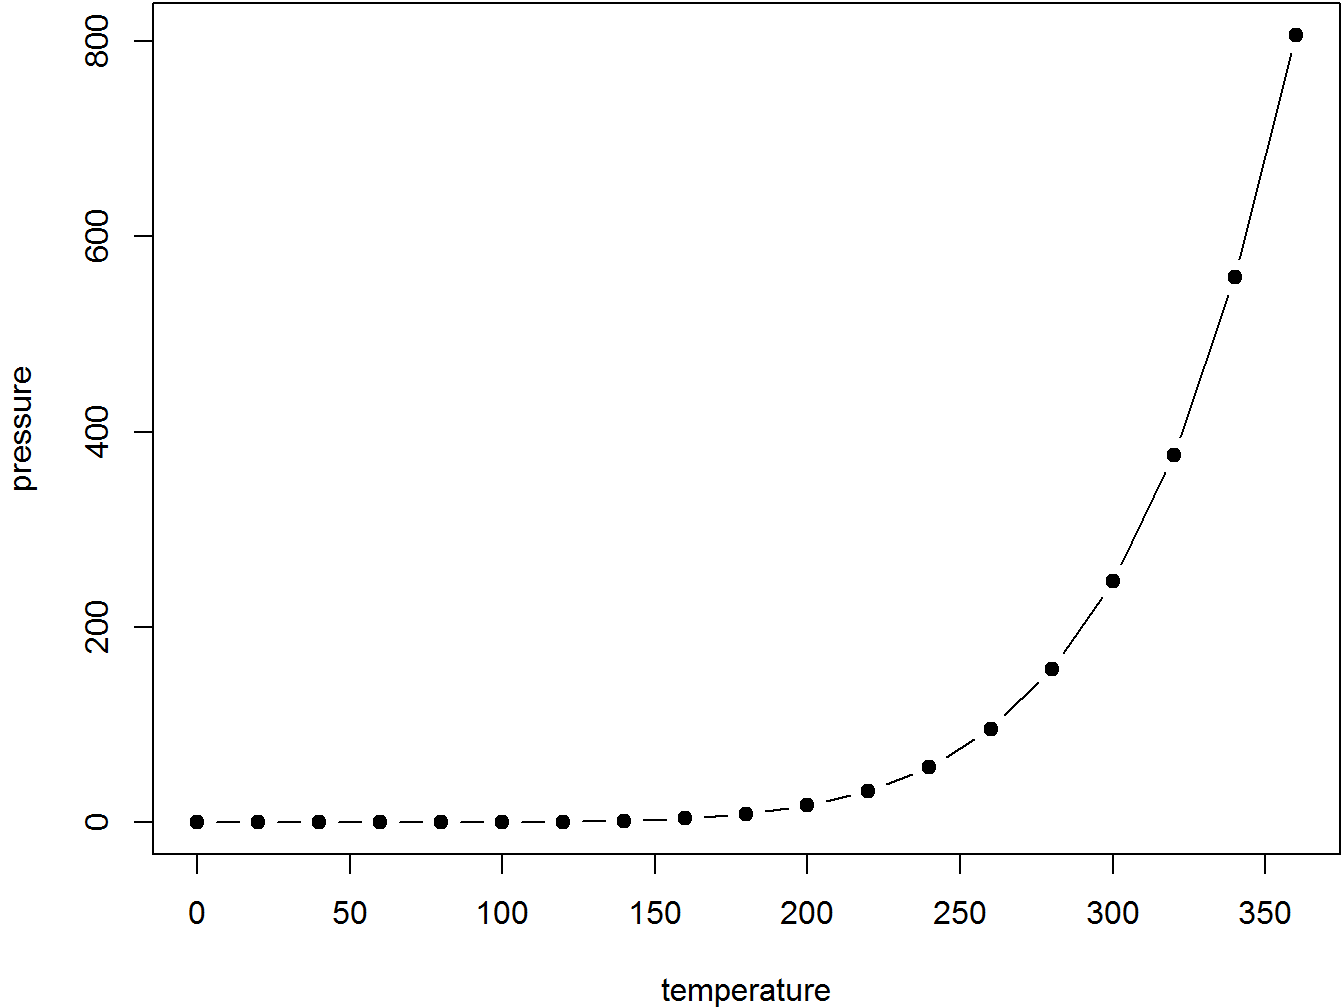
\includegraphics[width=0.8\linewidth]{context_files/figure-latex/nice-fig-1} 

}

\caption{Here is a nice figure!}\label{fig:nice-fig}
\end{figure}

Reference a figure by its code chunk label with the \texttt{fig:}
prefix, e.g., see Figure \ref{fig:nice-fig}. Similarly, you can
reference tables generated from \texttt{knitr::kable()}, e.g., see Table
\ref{tab:nice-tab}.

\begin{Shaded}
\begin{Highlighting}[]
\NormalTok{knitr::}\KeywordTok{kable}\NormalTok{(}
  \KeywordTok{head}\NormalTok{(iris, }\DecValTok{20}\NormalTok{), }\DataTypeTok{caption =} \StringTok{'Here is a nice table!'}\NormalTok{,}
  \DataTypeTok{booktabs =} \OtherTok{TRUE}
\NormalTok{)}
\end{Highlighting}
\end{Shaded}

\begin{table}

\caption{\label{tab:nice-tab}Here is a nice table!}
\centering
\begin{tabular}[t]{rrrrl}
\toprule
Sepal.Length & Sepal.Width & Petal.Length & Petal.Width & Species\\
\midrule
5.1 & 3.5 & 1.4 & 0.2 & setosa\\
4.9 & 3.0 & 1.4 & 0.2 & setosa\\
4.7 & 3.2 & 1.3 & 0.2 & setosa\\
4.6 & 3.1 & 1.5 & 0.2 & setosa\\
5.0 & 3.6 & 1.4 & 0.2 & setosa\\
\addlinespace
5.4 & 3.9 & 1.7 & 0.4 & setosa\\
4.6 & 3.4 & 1.4 & 0.3 & setosa\\
5.0 & 3.4 & 1.5 & 0.2 & setosa\\
4.4 & 2.9 & 1.4 & 0.2 & setosa\\
4.9 & 3.1 & 1.5 & 0.1 & setosa\\
\addlinespace
5.4 & 3.7 & 1.5 & 0.2 & setosa\\
4.8 & 3.4 & 1.6 & 0.2 & setosa\\
4.8 & 3.0 & 1.4 & 0.1 & setosa\\
4.3 & 3.0 & 1.1 & 0.1 & setosa\\
5.8 & 4.0 & 1.2 & 0.2 & setosa\\
\addlinespace
5.7 & 4.4 & 1.5 & 0.4 & setosa\\
5.4 & 3.9 & 1.3 & 0.4 & setosa\\
5.1 & 3.5 & 1.4 & 0.3 & setosa\\
5.7 & 3.8 & 1.7 & 0.3 & setosa\\
5.1 & 3.8 & 1.5 & 0.3 & setosa\\
\bottomrule
\end{tabular}
\end{table}

You can write citations, too. For example, we are using the
\textbf{bookdown} package \citep{R-bookdown} in this sample book, which
was built on top of R Markdown and \textbf{knitr} \citep{xie2015}.

\section{Complex surveys and statistical inference}\label{survey}

In this book we estimate measures of poverty and income concentration in
a populatiion, generaly of households or people, based on data colected
from a complex survey sample from the population, involving

1- different units selection probabilities;

2- clustering of units;

3- stratification of clusters, and

4- reweighting to compensate missing values and other adjustments.

Items 1 and 4 imply that we should use different units weights to avoid
biases when performing statistical analysis. Also, when estimating
variances, we should consider, not only the design weights but all
listed design characteristics 1-4.

In order to take into account the sample design characteristics it
should be used a specialized software like the R library
\textbf{survey}, adopted in this book.

\section{Linearization}\label{linearization}

Some measures of poverty and income concentration are defined by
non-differentiable functions so that it is not possible to use Taylor
linearization to estimate their variances. An alternative is to use
\textbf{Influence functions} as described in \citep{deville1999} and
\citep{osier2009}. The library convey implements this methodology to
work with \texttt{survey.design} objects and also with
\texttt{svyrep.design} objects.

Some examples of these measures are:

\begin{itemize}
\item
  At-risk-of-poverty threshold: \(arpt=.60q_{.50}\) where \(q_{.50}\) is
  the income median;
\item
  At-risk-of-poverty rate \(arpr=\frac{\sum_U 1(y_i \leq arpt)}{N}.100\)
\item
  Quintile share ratio
\end{itemize}

\(qsr=\frac{\sum_U 1(y_i>q_{.80})}{\sum_U 1(y_i\leq q_{.20})}\)

\begin{itemize}
\tightlist
\item
  Gini coefficient \(1+G=\frac{2\sum_U (r_i-1)y_i}{N\sum_Uy_i}\) where
  \(r_i\) is the rank of \(y_i\).
\end{itemize}

Note that it is not possible to use Taylor linearization for these
measures because they depend on quantiles and the Gini is defined as a
function of ranks. This could be done using the approach proposed by
Deville (1999) based upon influence functions.

\section{Influence function}\label{influence-function}

Let \(U\) be a population of size \(N\) and \(M\) be a measure that
allocates mass one to the set composed by one unit, that is
\(M(i)=M_i= 1\) if \(i\in U\) and \(M(i)=0\) if \(i\notin U\)

Now, a population parameter \(\theta\) can be expressed as a functional
of \(M\) \(\theta=T(M)\)

Examples of such parameters are:

\begin{itemize}
\item
  Total: \(Y=\sum_Uy_i=\sum_U y_iM_i=\int ydM=T(M)\)
\item
  Ratio of two totals:
  \(R=\frac{Y}{X}=\frac{\int y dM}{\int x dM}=T(M)\)
\item
  Cumulative distribution function:
  \(F(x)=\frac{\sum_U 1(y_i\leq x)}{N}=\frac{\int 1(y\leq x)dM}{\int{dM}}=T(M)\)
\end{itemize}

To estimate these parameters from the sample, we replace the measure
\(M\) by the estimated measure \(\hat{M}\) defined by:
\(\hat{M}(i)=\hat{M}_i= w_i\) if \(i\in s\) and \(\hat{M}(i)=0\) if
\(i\notin s\).

The estimators of the population parameters can then be expressed as
functional of the measure \(\hat{M}\).

\begin{itemize}
\item
  Total: \(\hat{Y}=T(\hat{M})=\int yd\hat{M}=\sum_s w_iy_i\)
\item
  Ratio of totals:
  \(\hat{R}=T(\hat{M})=\frac{\int y d\hat{M}}{\int x d\hat{M}}=\frac{\sum_s w_iy_i}{\sum_s w_ix_i}\)
\item
  Cumulative distribution function:
  \(\hat{F}(x)=T(\hat{M})=\frac{\int 1(y\leq x)d\hat{M}}{\int{d\hat{M}}}=\frac{\sum_s w_i 1(y_i\leq x)}{\sum_s w_i}\)
\end{itemize}

\section{The variance estimator}\label{the-variance-estimator}

The variance of the estimator \(T(\hat{M})\) can approximated by:

\[Var\left[T(\hat{M})\right]\cong var\left[\sum_s w_i z_i\right]\]

The \texttt{linearized} variable \(z\) is given by the derivative of the
functional:

\[
z_k=lim_{t\rightarrow0}\frac{T(M+t\delta_k)-T(M)}{t}=IT_k(M)
\]

where, \(\delta_k\) is the Dirac measure in \(k\): \(\delta_k(i)=1\) if
and only if \(i=k\).

This \textbf{derivative} is called \textbf{Influence Function} and was
introduced in the area of \textbf{Robust Statistics}.

\section{Influence functions -
Examples}\label{influence-functions---examples}

\begin{itemize}
\item
  Total: \[
  \begin{aligned}
  IT_k(M)&=lim_{t\rightarrow 0}\frac{T(M+t\delta_k)-T(M)}{t}\\
  &=lim_{t\rightarrow 0}\frac{\int y.d(M+t\delta_k)-\int y.dM}{t}\\
  &=lim_{t\rightarrow 0}\frac{\int yd(t\delta_k)}{t}=y_k  
  \end{aligned}
  \]
\item
  Ratio of two totals: \[
  \begin{aligned}
  IR_k(M)&=I\left(\frac{U}{V}\right)_k(M)=\frac{V(M)\times IU_k(M)-U(M)\times IV_k(M)}{V(M)^2}\\
  &=\frac{X y_k-Y x_k}{X^2}=\frac{1}{X}(y_k-Rx_k)
  \end{aligned}
  \]
\end{itemize}

\section{Linearization by influence function -
Examples}\label{linearization-by-influence-function---examples}

\begin{itemize}
\tightlist
\item
  At-risk-of-poverty threshold: \[
  arpt = 0.6\times m
  \] where \(m\) is the median income.
\end{itemize}

\[
z_k= -\frac{0.6}{f(m)}\times\frac{1}{N}\times\left[I(y_k\leq m-0.5) \right]
\]

\begin{itemize}
\tightlist
\item
  At-risk-of-poverty rate:
\end{itemize}

\[
 arpr=\frac{\sum_U I(y_i \leq t)}{\sum_U w_i}.100
\] \[
z_k=\frac{1}{N}\left[I(y_k\leq t)-t\right]-\frac{0.6}{N}\times\frac{f(t)}{f(m)}\left[I(y_k\leq m)-0.5\right]
\]

where:

\(N\) - population size;

\(t\) - at-risk-of-poverty threshold;

\(y_k\) - income of person \(k\);

\(m\) - median income;

\(f\) - income density function;

\section{Structure of the library}\label{structure-of-the-library}

In the library convey, there are some basic functions that produces the
linearized variables of some estimates that often enter in the
definition of measures of concentration and poverty. For example the
\texttt{quantile} which is linearized by the function
\texttt{svyiqalpha}. Other example is the function \texttt{svyisq} that
linearizes the total below a quantile of the variable.

From the linearized variables of these basic estimates it is possible by
using rules of composition, valid for influence functions, to derive the
influence function of more complex estimates. By definition the
influence function is a Gateaux derivative and the rules rules of
composition valid for Gateaux derivatives also hold for Influence
Functions.

The following property of Gateaux derivatives was often used in the
library convey. Let \(g\) be a differentible function of \(m\)
variables. Suppose we want to compute the influence function of the
estimator \(g(T_1, T_2,\ldots, T_m)\), knowing the Influence function of
the estimators \(T_i, i=1,\ldots, m\). Then the following holds:

\[
I(g(T_1, T_2,\ldots, T_m)) = \sum_{i=1}^m \frac{\partial g}{\partial T_i}I(T_i)
\]

In the library convey this rule is implemented by the function
\texttt{contrastinf} which uses the R function \texttt{deriv} to compute
the formal partial derivatives \(\frac{\partial g}{\partial T_i}\).

For example, suppose we want to linearize the
\texttt{Relative\ median\ poverty\ gap}(rmpg), defined as the difference
between the at-risk-of-poverty threshold (\texttt{arpt}) and the median
of incomes less than the \texttt{arpt} relative to the \texttt{arprt}:

\[
rmpg= \frac{arpt-medpoor} {arpt}
\]

where \texttt{medpoor} is the median of incomes less than \texttt{arpt}.

Suppose we know how to linearize \texttt{arpt} and \texttt{medpoor},
then by applying the function \texttt{contrastinf} with \[
g(T_1,T_2)= \frac{(T_1 - T_2)}{T_1}
\] we linearize the \texttt{rmpg}.

\subsection{Examples of use of the library
convey}\label{examples-of-use-of-the-library-convey}

In the following examples we will use the data set \texttt{eusilc}
contained in the libraries \texttt{vardpoor} and \texttt{Laeken}.

\begin{Shaded}
\begin{Highlighting}[]
\KeywordTok{library}\NormalTok{(vardpoor)}
\KeywordTok{data}\NormalTok{(eusilc)}
\end{Highlighting}
\end{Shaded}

Next, we create an object of class \texttt{survey.design} using the
function \texttt{svydesign} of the library survey:

\begin{Shaded}
\begin{Highlighting}[]
\KeywordTok{library}\NormalTok{(survey)}
\NormalTok{des_eusilc <-}\StringTok{ }\KeywordTok{svydesign}\NormalTok{(}\DataTypeTok{ids =} \NormalTok{~rb030, }\DataTypeTok{strata =}\NormalTok{~db040,  }\DataTypeTok{weights =} \NormalTok{~rb050, }\DataTypeTok{data =} \NormalTok{eusilc)}
\end{Highlighting}
\end{Shaded}

Right after the creation of the design object \texttt{des\_eusilc}, we
should use the function \texttt{convey\_prep} that adds an attribute to
the survey design which saves information on the design object based
upon the whole sample, needed to work with subset designs.

\begin{Shaded}
\begin{Highlighting}[]
\KeywordTok{library}\NormalTok{(convey)}
\NormalTok{des_eusilc <-}\StringTok{ }\KeywordTok{convey_prep}\NormalTok{( des_eusilc )}
\end{Highlighting}
\end{Shaded}

To estimate the \texttt{at-risk-of-poverty\ rate} we use the function
\texttt{svyarpt}:

\begin{Shaded}
\begin{Highlighting}[]
\KeywordTok{svyarpr}\NormalTok{(~eqIncome, }\DataTypeTok{design=}\NormalTok{des_eusilc)}
\end{Highlighting}
\end{Shaded}

\begin{verbatim}
            arpr     SE
eqIncome 0.14444 0.0028
\end{verbatim}

To estimate the \texttt{at-risk-of-poverty\ rate} for domains defined by
the variable \texttt{db040} we use

\begin{Shaded}
\begin{Highlighting}[]
\KeywordTok{svyby}\NormalTok{(~eqIncome, }\DataTypeTok{by =} \NormalTok{~db040, }\DataTypeTok{design =} \NormalTok{des_eusilc, }\DataTypeTok{FUN =} \NormalTok{svyarpr, }\DataTypeTok{deff =} \OtherTok{FALSE}\NormalTok{)}
\end{Highlighting}
\end{Shaded}

\begin{verbatim}
                      db040  eqIncome          se
Burgenland       Burgenland 0.1953984 0.017202243
Carinthia         Carinthia 0.1308627 0.010610622
Lower Austria Lower Austria 0.1384362 0.006517660
Salzburg           Salzburg 0.1378734 0.011579280
Styria               Styria 0.1437464 0.007452360
Tyrol                 Tyrol 0.1530819 0.009880430
Upper Austria Upper Austria 0.1088977 0.005928336
Vienna               Vienna 0.1723468 0.007682826
Vorarlberg       Vorarlberg 0.1653731 0.013754670
\end{verbatim}

Using the same data set, we estimate the
\texttt{quintile\ share\ ratio}:

\begin{Shaded}
\begin{Highlighting}[]
\CommentTok{# for the whole population}
\KeywordTok{svyqsr}\NormalTok{(~eqIncome, }\DataTypeTok{design=}\NormalTok{des_eusilc, }\DataTypeTok{alpha=} \NormalTok{.}\DecValTok{20}\NormalTok{)}
\end{Highlighting}
\end{Shaded}

\begin{verbatim}
          qsr     SE
eqIncome 3.97 0.0426
\end{verbatim}

\begin{Shaded}
\begin{Highlighting}[]
\CommentTok{# for domains}
\KeywordTok{svyby}\NormalTok{(~eqIncome, }\DataTypeTok{by =} \NormalTok{~db040, }\DataTypeTok{design =} \NormalTok{des_eusilc,}
  \DataTypeTok{FUN =} \NormalTok{svyqsr, }\DataTypeTok{alpha=} \NormalTok{.}\DecValTok{20}\NormalTok{, }\DataTypeTok{deff =} \OtherTok{FALSE}\NormalTok{)}
\end{Highlighting}
\end{Shaded}

\begin{verbatim}
                      db040 eqIncome         se
Burgenland       Burgenland 5.008486 0.32755685
Carinthia         Carinthia 3.562404 0.10909726
Lower Austria Lower Austria 3.824539 0.08783599
Salzburg           Salzburg 3.768393 0.17015086
Styria               Styria 3.464305 0.09364800
Tyrol                 Tyrol 3.586046 0.13629739
Upper Austria Upper Austria 3.668289 0.09310624
Vienna               Vienna 4.654743 0.13135731
Vorarlberg       Vorarlberg 4.366511 0.20532075
\end{verbatim}

These functions can be used as S3 methods for the classes
\texttt{survey.design} and \texttt{svyrep.design}.

Let's create a design object of class \texttt{svyrep.design} and run the
function \texttt{convey\_prep} on it:

\begin{Shaded}
\begin{Highlighting}[]
\NormalTok{des_eusilc_rep <-}\StringTok{ }\KeywordTok{as.svrepdesign}\NormalTok{(des_eusilc, }\DataTypeTok{type =} \StringTok{"bootstrap"}\NormalTok{)}
\NormalTok{des_eusilc_rep <-}\StringTok{ }\KeywordTok{convey_prep}\NormalTok{(des_eusilc_rep) }
\end{Highlighting}
\end{Shaded}

and then use the function \texttt{svyarpr}:

\begin{Shaded}
\begin{Highlighting}[]
\KeywordTok{svyarpr}\NormalTok{(~eqIncome, }\DataTypeTok{design=}\NormalTok{des_eusilc_rep)}
\end{Highlighting}
\end{Shaded}

\begin{verbatim}
            arpr     SE
eqIncome 0.14444 0.0026
\end{verbatim}

\begin{Shaded}
\begin{Highlighting}[]
\KeywordTok{svyby}\NormalTok{(~eqIncome, }\DataTypeTok{by =} \NormalTok{~db040, }\DataTypeTok{design =} \NormalTok{des_eusilc_rep, }\DataTypeTok{FUN =} \NormalTok{svyarpr, }\DataTypeTok{deff =} \OtherTok{FALSE}\NormalTok{)}
\end{Highlighting}
\end{Shaded}

\begin{verbatim}
                      db040  eqIncome se.eqIncome
Burgenland       Burgenland 0.1953984 0.018160170
Carinthia         Carinthia 0.1308627 0.012136183
Lower Austria Lower Austria 0.1384362 0.007689382
Salzburg           Salzburg 0.1378734 0.013658170
Styria               Styria 0.1437464 0.007331796
Tyrol                 Tyrol 0.1530819 0.010196732
Upper Austria Upper Austria 0.1088977 0.006773692
Vienna               Vienna 0.1723468 0.006875140
Vorarlberg       Vorarlberg 0.1653731 0.014161893
\end{verbatim}

The functions of the library convey are called in a similar way to the
functions in library survey.

It is also possible to deal with missing values by using the argument
\texttt{na.rm}.

\begin{Shaded}
\begin{Highlighting}[]
\CommentTok{# survey.design using a variable with missings}
\KeywordTok{svygini}\NormalTok{( ~}\StringTok{ }\NormalTok{py010n , }\DataTypeTok{design =} \NormalTok{des_eusilc )}
\end{Highlighting}
\end{Shaded}

\begin{verbatim}
       gini SE
py010n   NA NA
\end{verbatim}

\begin{Shaded}
\begin{Highlighting}[]
\KeywordTok{svygini}\NormalTok{( ~}\StringTok{ }\NormalTok{py010n , }\DataTypeTok{design =} \NormalTok{des_eusilc , }\DataTypeTok{na.rm =} \OtherTok{TRUE} \NormalTok{)}
\end{Highlighting}
\end{Shaded}

\begin{verbatim}
          gini     SE
py010n 0.64606 0.0036
\end{verbatim}

\begin{Shaded}
\begin{Highlighting}[]
\CommentTok{# svyrep.design using a variable with missings}
\CommentTok{# svygini( ~ py010n , design = des_eusilc_rep ) get error}
\KeywordTok{svygini}\NormalTok{( ~}\StringTok{ }\NormalTok{py010n , }\DataTypeTok{design =} \NormalTok{des_eusilc_rep , }\DataTypeTok{na.rm =} \OtherTok{TRUE} \NormalTok{)}
\end{Highlighting}
\end{Shaded}

\begin{verbatim}
          gini     SE
py010n 0.64606 0.0031
\end{verbatim}

djalma, where do these references go on this page? \citep{berger2003}
and \citep{osier2009} and \citep{deville1999}

\chapter{Poverty Indices}\label{poverty}

{[}I think this is a good start. I don't think that gender pay gap,
quantiles and totals are measures of poverty. Consider another chapter
on other wellbeing measures.{]} this is a test \#\# At Risk of Poverty
Ratio and Threshold (svyarpr, svyarpt)

here are the references

\citep{osier2009} and \citep{deville1999}

\section{The Gender Pay Gap (svygpg)}\label{the-gender-pay-gap-svygpg}

here are the references

\citep{osier2009} and \citep{deville1999}

\section{Quintile Share Ratio
(svyqsr)}\label{quintile-share-ratio-svyqsr}

here are the references

\citep{osier2009} and \citep{deville1999}

\section{Relative Median Income Ratio
(svyrmir)}\label{relative-median-income-ratio-svyrmir}

here are the references

\citep{osier2009} and \citep{deville1999}

\section{Relative Median Poverty Gap
(svyrmpg)}\label{relative-median-poverty-gap-svyrmpg}

here are the references

\citep{osier2009} and \citep{deville1999}

\section{Median Income Below the At Risk of Poverty Threshold
(svypoormed)}\label{median-income-below-the-at-risk-of-poverty-threshold-svypoormed}

here are the references

\citep{osier2009} and \citep{deville1999}

\section{Foster-Greer-Thorbecke class
(svyfgt)}\label{foster-greer-thorbecke-class-svyfgt}

here are the references

\citep{foster1984} and \citep{berger2003}

\citep{foster1984} proposed a family of indicators to measure poverty.

The class of \(FGT\) measures, can be defined as

\[
p=\frac{1}{N}\sum_{k\in U}h(y_{k},\theta ), 
\]

where

\[
h(y_{k},\theta )=\left[ \frac{(\theta -y_{k})}{\theta }\right] ^{\gamma
}\delta \left\{ y_{k}\leq \theta \right\} , 
\]

where: \(\theta\) is the poverty threshold; \(\delta\) the indicator
function that assigns value 1 if the condition \(\{y_{k}\leq \theta \}\)
is satisfied and 0 otherwise, and \(\gamma\) is a non-negative constant.

When \(\gamma =0\), \(p\) can be interpreted as the poverty headcount
ratio, and for \(\gamma \geq 1\), the weight of the income shortfall of
the poor to a power \(\gamma\), (Foster and all, 1984).

The poverty measure FGT is implemented in the library convey by the
function \texttt{svyfgt}. The argument \texttt{thresh\_type} of this
function defines the type of poverty threshold adopted. There are three
possible choices:

\begin{enumerate}
\def\labelenumi{\arabic{enumi}.}
\tightlist
\item
  \texttt{abs} -- fixed and given by the argument thresh\_value
\item
  \texttt{relq} -- a proportion of a quantile fixed by the argument
  \texttt{proportion} and the quantile is defined by the argument
  \texttt{order}.
\item
  \texttt{relm} -- a proportion of the mean fixed the argument
  \texttt{proportion}
\end{enumerate}

The quantile and the mean involved in the definition of the threshold
are estimated for the whole population. When \(\gamma=0\) and
\(\theta= .6*MED\) the measure is equal to the indicator \texttt{arpr}
computed by the function \texttt{svyarpr}.

Next, we give some examples of the function \texttt{svyfgt} to estimate
the values of the FGT poverty index.

Consider first the poverty threshold fixed (\(\gamma=0\)) in the value
\(10000\). The headcount ratio (FGT0) is

\begin{Shaded}
\begin{Highlighting}[]
\KeywordTok{svyfgt}\NormalTok{(~eqIncome, des_eusilc, }\DataTypeTok{g=}\DecValTok{0}\NormalTok{, }\DataTypeTok{abs_thresh=}\DecValTok{10000}\NormalTok{)}
\end{Highlighting}
\end{Shaded}

\begin{verbatim}
            fgt0     SE
eqIncome 0.11444 0.0027
\end{verbatim}

The poverty gap (FGT1) (\(\gamma=1\)) index for the poverty threshold
fixed at the same value is

\begin{Shaded}
\begin{Highlighting}[]
\KeywordTok{svyfgt}\NormalTok{(~eqIncome, des_eusilc, }\DataTypeTok{g=}\DecValTok{1}\NormalTok{, }\DataTypeTok{abs_thresh=}\DecValTok{10000}\NormalTok{)}
\end{Highlighting}
\end{Shaded}

\begin{verbatim}
             fgt1     SE
eqIncome 0.032085 0.0011
\end{verbatim}

To estimate the FGT0 with the poverty threshold fixed at \(0.6* MED\) we
fix the argument type\_thresh=``relq'' and use the default values for
\texttt{percent} and \texttt{order}:

\begin{Shaded}
\begin{Highlighting}[]
\KeywordTok{svyfgt}\NormalTok{(~eqIncome, des_eusilc, }\DataTypeTok{g=}\DecValTok{0}\NormalTok{, }\DataTypeTok{type_thresh=} \StringTok{"relq"}\NormalTok{)}
\end{Highlighting}
\end{Shaded}

\begin{verbatim}
            fgt0     SE
eqIncome 0.14444 0.0028
\end{verbatim}

that matches the estimate obtained by

\begin{Shaded}
\begin{Highlighting}[]
\KeywordTok{svyarpr}\NormalTok{(~eqIncome, }\DataTypeTok{design=}\NormalTok{des_eusilc, .}\DecValTok{5}\NormalTok{, .}\DecValTok{6}\NormalTok{)}
\end{Highlighting}
\end{Shaded}

\begin{verbatim}
            arpr     SE
eqIncome 0.14444 0.0028
\end{verbatim}

To estimate the poverty gap(FGT1) with the poverty threshold equal to
\(0.6*MEAN\) we use:

\begin{Shaded}
\begin{Highlighting}[]
\KeywordTok{svyfgt}\NormalTok{(~eqIncome, des_eusilc, }\DataTypeTok{g=}\DecValTok{1}\NormalTok{, }\DataTypeTok{type_thresh=} \StringTok{"relm"}\NormalTok{)}
\end{Highlighting}
\end{Shaded}

\begin{verbatim}
             fgt1     SE
eqIncome 0.051187 0.0011
\end{verbatim}

\chapter{Inequality Measurement}\label{inequality}

\section{Lorenz Curve (svylorenz)}\label{lorenz-curve-svylorenz}

Though not an inequality measure in itself, the Lorenz curve is a
classic instrument of distribution analysis. Basically, it is a function
that associates a cumulative share of the population and the share of
the total income it owns. In mathematical terms,

\[
L(p) = \frac{\int_{-\infty}^{Q_p}yf(y)dy}{\int_{-\infty}^{+\infty}yf(y)dy}
\]

where \(Q_p\) is the quantile \(p\) of the population.

The two extreme distributive cases are

\begin{itemize}
\tightlist
\item
  Perfect equality:

  \begin{itemize}
  \tightlist
  \item
    Every individual has the same income;
  \item
    Every share of the population has the same share of the income;
  \item
    Therefore, the reference curve is
    \[L(p) = p \text{ } \forall p \in [0,1] \text{.}\].
  \end{itemize}
\item
  Perfect inequality:

  \begin{itemize}
  \tightlist
  \item
    One individual concentrates all of society's income, while the other
    individuals have zero income;
  \item
    Therefore, the reference curve is
  \end{itemize}
\end{itemize}

\[
L(p)=
\begin{cases}
0, &\forall p < 1 \\
1, &\text{if } p = 1 \text{.}
\end{cases}
\]

In order to evaluate the degree of inequality in a society, the analyst
looks at the distance between the real curve and those two reference
curves.

The estimator of this function was derived by \citep{kovacevic1997}:

\[
L(p) = \frac{ \sum_{i \in S} w_i \cdot y_i \cdot \delta \{ y_i \le \widehat{Q}_p \}}{\widehat{Y}}, \text{ } 0 \le p \le 1.
\]

Yet, this formula is used to calculate specific points of the curve and
their respective SEs. The formula to plot an approximation of the
continuous empirical curve comes from \citep{lerman1989}.

\section{Measures derived from the Lorenz
Curve}\label{measures-derived-from-the-lorenz-curve}

\subsection{Gini index (svygini)}\label{gini-index-svygini}

The Gini index is an attempt to express the inequality presented in the
Lorenz curve as a single number. In essence, the Gini index is twice the
area between the equality curve and the real Lorenz curve. Put simply:

\[
\begin{aligned}
G &= 2 \bigg( \int_{0}^{1} pdp - \int_{0}^{1} L(p)dp \bigg) \\
\therefore G &= 1 - 2 \int_{0}^{1} L(p)dp
\end{aligned}
\]

where \(G=0\) in case of perfect equality and \(G = 1\) in the case of
perfect inequality.

The estimator proposed by \citep{osier2009} is defined as:

\[
\widehat{G} = \frac{ 2 \sum_{i \in S} w_i r_i y_i - \sum_{i \in S} w_i y_i }{ \hat{Y} }
\]

The linearized formula of \(\widehat{G}\) is used to calculate the SE.

\subsection{Amato index (svyamato)}\label{amato-index-svyamato}

The Amato index is also based on the Lorenz curve, but instead of
focusing on the area of the curve, it focuses on its length.
\citep{arnold2012} proposes a formula not directly based in the Lorenz
curve, which \citep{barabesi2016} uses to present the following
estimator:

\[
\widehat{A} = \sum_{i \in S} w_i \bigg[ \frac{1}{\widehat{N}^2} + \frac{y_i^2}{\widehat{Y}^2} \bigg]^{\frac{1}{2}} \text{,}
\]

which also generates the linearized formula for SE estimation.

The minimum value \(A\) assumes is \(\sqrt{2}\) and the maximum is
\(2\). In order to get a measure in the interval \([0,1]\), the
standardized Amato index \(\widetilde{A}\) can be defined as:

\[
\widetilde{A} = \frac{ A - \sqrt{2} }{2 - \sqrt{2} } \text{ .}
\]

\subsection{Zenga Index and Curve (svyzenga,
svyzengacurve)}\label{zenga-index-and-curve-svyzenga-svyzengacurve}

The Zenga index and its curve were proposed in \citep{zenga2007}. As
\citep{polisicchio2011} noticed, this curve derives directly from the
Lorenz curve, and can be defined as:

\[
Z(p) = 1 - \frac{L(p)}{p} \cdot \frac{1 - p}{1 - L(p)}.
\]

In the \texttt{convey} library, an experimental estimator based on the
Lorenz curve is used:

\[
\widehat{Z(p)} = \frac{ p \widehat{Y} - \widehat{\widetilde{Y}}(p) }{p \big[ \widehat{Y} - \widehat{\widetilde{Y}}(p) \big] }.
\]

In turn, the Zenga index derives from this curve and is defined as:

\[
Z = \int_0^1 Z(p)dp.
\]

However, its estimators were proposed by \citep{langel2012} and
\citep{barabesi2016}. In this library, the latter is used and is defined
as:

\[
\widehat{Z} = 1 - \sum_{i \in S} w_i \bigg[ \frac{ ( \widehat{N} - \widehat{H}_{y_i} ) ( \widehat{Y} -\widehat{K}_{y_i} ) }
{ \widehat{N} \cdot \widehat{H}_{y_i} \cdot \widehat{K}_{y_i} } \bigg]
\]

where \(\widehat{N}\) is the population total, \(\widehat{Y}\) is the
total income, \(\widehat{H}_{y_i}\) is the sum of incomes below or equal
to \(y_i\) and \(\widehat{N}_{y_i}\) is the sum of incomes greater or
equal to \(y_i\).

\section{Entropy-based Measures}\label{entropy-based-measures}

\subsection{Atkinson index (svyatk)}\label{atkinson-index-svyatk}

here are the references

\citep{langel2012} and \citep{biewen2003}

\subsection{Generalized Entropy and Decomposition (svygei,
svygeidec)}\label{generalized-entropy-and-decomposition-svygei-svygeidec}

guilherme..this has three references? not just two?

here are the references

\citep{langel2012} and \citep{biewen2003} and \citep{shorrocks1984}

\subsection{J-Divergence Entropy and Decomposition (svyjdiv,
svyjdivdec)}\label{j-divergence-entropy-and-decomposition-svyjdiv-svyjdivdec}

here are the references

\citep{shorrocks1984} and \citep{rohde2016} and \citep{biewen2003}

\subsection{Rényi Divergence
(svyrenyi)}\label{renyi-divergence-svyrenyi}

here are the references

\citep{langel2012}

\chapter{Multidimensional Indices}\label{multidimensional}

\section{Alkire-Foster Class and Decomposition (svyafc,
svyafcdec)}\label{alkire-foster-class-and-decomposition-svyafc-svyafcdec}

In November 2015, Christopher Jindra presented at the Oxford Poverty and
Human Development Initiative on the Alkire-Foster multidimensional
poverty measure. His presentation can be viewed
\href{http://www.ophi.org.uk/wp-content/uploads/Jindra_151109_OPHISeminar.pdf}{here}.
The example below reproduces those statistics.

Load and prepare the same data set:

\begin{Shaded}
\begin{Highlighting}[]
\CommentTok{# load the convey package}
\KeywordTok{library}\NormalTok{(convey)}

\CommentTok{# load the survey library}
\KeywordTok{library}\NormalTok{(survey)}

\CommentTok{# load the stata-style webuse library}
\KeywordTok{library}\NormalTok{(webuse)}

\CommentTok{# load the same microdata set used by Jindra in his presentation}
\KeywordTok{webuse}\NormalTok{(}\StringTok{"nlsw88"}\NormalTok{)}

\CommentTok{# coerce that `tbl_df` to a standard R `data.frame`}
\NormalTok{nlsw88 <-}\StringTok{ }\KeywordTok{data.frame}\NormalTok{( nlsw88 )}

\CommentTok{# create a `collgrad` column}
\NormalTok{nlsw88$collgrad <-}
\StringTok{    }\KeywordTok{factor}\NormalTok{( }
        \KeywordTok{as.numeric}\NormalTok{( nlsw88$collgrad ) , }
        \DataTypeTok{label =} \KeywordTok{c}\NormalTok{( }\StringTok{'not college grad'} \NormalTok{, }\StringTok{'college grad'} \NormalTok{) , }
        \DataTypeTok{ordered =} \OtherTok{TRUE} 
      \NormalTok{)}

\CommentTok{# initiate a linearized survey design object}
\NormalTok{des_nlsw88 <-}\StringTok{ }\KeywordTok{svydesign}\NormalTok{( }\DataTypeTok{ids =} \NormalTok{~}\DecValTok{1} \NormalTok{, }\DataTypeTok{data =} \NormalTok{nlsw88 )}

\CommentTok{# immediately run the `convey_prep` function on the survey design}
\NormalTok{des_nlsw88 <-}\StringTok{ }\KeywordTok{convey_prep}\NormalTok{(des_nlsw88)}
\end{Highlighting}
\end{Shaded}

Replicate PDF page 9

\begin{Shaded}
\begin{Highlighting}[]
\NormalTok{page_nine <-}
\StringTok{  }\KeywordTok{svyafc}\NormalTok{(}
    \NormalTok{~}\StringTok{ }\NormalTok{wage +}\StringTok{ }\NormalTok{collgrad +}\StringTok{ }\NormalTok{hours , }
    \DataTypeTok{design =} \NormalTok{des_nlsw88 , }
    \DataTypeTok{cutoffs =} \KeywordTok{list}\NormalTok{( }\DecValTok{4}\NormalTok{, }\StringTok{'college grad'} \NormalTok{, }\DecValTok{26} \NormalTok{) , }
    \DataTypeTok{k =} \DecValTok{1}\NormalTok{/}\DecValTok{3} \NormalTok{, }\DataTypeTok{g =} \DecValTok{0} \NormalTok{, }
    \DataTypeTok{na.rm =} \OtherTok{TRUE}
  \NormalTok{)}

\CommentTok{# MO and seMO}
\KeywordTok{print}\NormalTok{( page_nine )}
\end{Highlighting}
\end{Shaded}

\begin{verbatim}
##      alkire-foster     SE
## [1,]       0.36991 0.0053
\end{verbatim}

\begin{Shaded}
\begin{Highlighting}[]
\CommentTok{# H seH and A seA}
\KeywordTok{print}\NormalTok{( }\KeywordTok{attr}\NormalTok{( page_nine , }\StringTok{"extra"} \NormalTok{) )}
\end{Highlighting}
\end{Shaded}

\begin{verbatim}
##        coef          SE
## H 0.8082070 0.008316807
## A 0.4576895 0.004573443
\end{verbatim}

Replicate PDF page 10

\begin{Shaded}
\begin{Highlighting}[]
\NormalTok{page_ten <-}\StringTok{ }\OtherTok{NULL}

\CommentTok{# loop through every poverty cutoff `k`}
\NormalTok{for( ks in }\KeywordTok{seq}\NormalTok{( }\FloatTok{0.1} \NormalTok{, }\DecValTok{1} \NormalTok{, .}\DecValTok{1} \NormalTok{) )\{}
    
    \NormalTok{this_ks <-}
\StringTok{        }\KeywordTok{svyafc}\NormalTok{(}
            \NormalTok{~}\StringTok{ }\NormalTok{wage +}\StringTok{ }\NormalTok{collgrad +}\StringTok{ }\NormalTok{hours , }
            \DataTypeTok{design =} \NormalTok{des_nlsw88 , }
            \DataTypeTok{cutoffs =} \KeywordTok{list}\NormalTok{( }\DecValTok{4} \NormalTok{, }\StringTok{'college grad'} \NormalTok{, }\DecValTok{26} \NormalTok{) , }
            \DataTypeTok{k =} \NormalTok{ks , }
            \DataTypeTok{g =} \DecValTok{0} \NormalTok{, }
            \DataTypeTok{na.rm =} \OtherTok{TRUE} 
           \NormalTok{)}
    
    \NormalTok{page_ten <-}
\StringTok{        }\KeywordTok{rbind}\NormalTok{(}
            \NormalTok{page_ten ,}
            \KeywordTok{data.frame}\NormalTok{( }
                \DataTypeTok{k =} \NormalTok{ks , }
                \DataTypeTok{MO =} \KeywordTok{coef}\NormalTok{( this_ks ) ,}
                \DataTypeTok{seMO =} \KeywordTok{SE}\NormalTok{( this_ks ) ,}
                \DataTypeTok{H =} \KeywordTok{attr}\NormalTok{( this_ks , }\StringTok{"extra"} \NormalTok{)[ }\DecValTok{1} \NormalTok{, }\DecValTok{1} \NormalTok{] ,}
                \DataTypeTok{seH =} \KeywordTok{attr}\NormalTok{( this_ks , }\StringTok{"extra"} \NormalTok{)[ }\DecValTok{1} \NormalTok{, }\DecValTok{2} \NormalTok{] ,}
                \DataTypeTok{A =} \KeywordTok{attr}\NormalTok{( this_ks , }\StringTok{"extra"} \NormalTok{)[ }\DecValTok{2} \NormalTok{, }\DecValTok{1} \NormalTok{] ,}
                \DataTypeTok{seA =} \KeywordTok{attr}\NormalTok{( this_ks , }\StringTok{"extra"} \NormalTok{)[ }\DecValTok{2} \NormalTok{, }\DecValTok{2} \NormalTok{]}
          \NormalTok{)}
        \NormalTok{)}
    
\NormalTok{\}}

\NormalTok{knitr::}\KeywordTok{kable}\NormalTok{(}
  \NormalTok{page_ten , }\DataTypeTok{caption =} \StringTok{'Here is a nice table!'}\NormalTok{,}
  \DataTypeTok{booktabs =} \OtherTok{TRUE}
\NormalTok{)}
\end{Highlighting}
\end{Shaded}

\begin{table}

\caption{\label{tab:unnamed-chunk-19}Here is a nice table!}
\centering
\begin{tabular}[t]{rrrrrrr}
\toprule
k & MO & seMO & H & seH & A & seA\\
\midrule
0.1 & 0.3699078 & 0.0053059 & 0.8082070 & 0.0083168 & 0.4576895 & 0.0045734\\
0.2 & 0.3699078 & 0.0053059 & 0.8082070 & 0.0083168 & 0.4576895 & 0.0045734\\
0.3 & 0.3699078 & 0.0053059 & 0.8082070 & 0.0083168 & 0.4576895 & 0.0045734\\
0.4 & 0.1865894 & 0.0068123 & 0.2582516 & 0.0092455 & 0.7225101 & 0.0051745\\
0.5 & 0.1865894 & 0.0068123 & 0.2582516 & 0.0092455 & 0.7225101 & 0.0051745\\
\addlinespace
0.6 & 0.1865894 & 0.0068123 & 0.2582516 & 0.0092455 & 0.7225101 & 0.0051745\\
0.7 & 0.0432649 & 0.0042978 & 0.0432649 & 0.0042978 & 1.0000000 & 0.0000000\\
0.8 & 0.0432649 & 0.0042978 & 0.0432649 & 0.0042978 & 1.0000000 & 0.0000000\\
0.9 & 0.0432649 & 0.0042978 & 0.0432649 & 0.0042978 & 1.0000000 & 0.0000000\\
1.0 & 0.0432649 & 0.0042978 & 0.0432649 & 0.0042978 & 1.0000000 & 0.0000000\\
\bottomrule
\end{tabular}
\end{table}

still need to replicate PDF page 13

\url{https://github.com/DjalmaPessoa/convey/issues/168}

then keep going replicating this

\url{https://github.com/DjalmaPessoa/convey/issues/154}

\citep{alkire2011} and \citep{alkire2015} and \citep{pacifico2016}

\section{Bourguignon (1999) inequality class
(svybmi)}\label{bourguignon-1999-inequality-class-svybmi}

\citep{bourguignon1999} and \citep{lugo2007}

\bibliography{packages,book}


\end{document}
